% Options for packages loaded elsewhere
\PassOptionsToPackage{unicode}{hyperref}
\PassOptionsToPackage{hyphens}{url}
%
\documentclass[
]{article}
\usepackage{lmodern}
\usepackage{amssymb,amsmath}
\usepackage{ifxetex,ifluatex}
\ifnum 0\ifxetex 1\fi\ifluatex 1\fi=0 % if pdftex
  \usepackage[T1]{fontenc}
  \usepackage[utf8]{inputenc}
  \usepackage{textcomp} % provide euro and other symbols
\else % if luatex or xetex
  \usepackage{unicode-math}
  \defaultfontfeatures{Scale=MatchLowercase}
  \defaultfontfeatures[\rmfamily]{Ligatures=TeX,Scale=1}
\fi
% Use upquote if available, for straight quotes in verbatim environments
\IfFileExists{upquote.sty}{\usepackage{upquote}}{}
\IfFileExists{microtype.sty}{% use microtype if available
  \usepackage[]{microtype}
  \UseMicrotypeSet[protrusion]{basicmath} % disable protrusion for tt fonts
}{}
\makeatletter
\@ifundefined{KOMAClassName}{% if non-KOMA class
  \IfFileExists{parskip.sty}{%
    \usepackage{parskip}
  }{% else
    \setlength{\parindent}{0pt}
    \setlength{\parskip}{6pt plus 2pt minus 1pt}}
}{% if KOMA class
  \KOMAoptions{parskip=half}}
\makeatother
\usepackage{xcolor}
\IfFileExists{xurl.sty}{\usepackage{xurl}}{} % add URL line breaks if available
\IfFileExists{bookmark.sty}{\usepackage{bookmark}}{\usepackage{hyperref}}
\hypersetup{
  pdftitle={Team mTurk - Motivating Quality Work},
  pdfauthor={Kevin Hanna, Kevin Stone, Changjing Zhao},
  hidelinks,
  pdfcreator={LaTeX via pandoc}}
\urlstyle{same} % disable monospaced font for URLs
\usepackage[margin=1in]{geometry}
\usepackage{color}
\usepackage{fancyvrb}
\newcommand{\VerbBar}{|}
\newcommand{\VERB}{\Verb[commandchars=\\\{\}]}
\DefineVerbatimEnvironment{Highlighting}{Verbatim}{commandchars=\\\{\}}
% Add ',fontsize=\small' for more characters per line
\usepackage{framed}
\definecolor{shadecolor}{RGB}{248,248,248}
\newenvironment{Shaded}{\begin{snugshade}}{\end{snugshade}}
\newcommand{\AlertTok}[1]{\textcolor[rgb]{0.94,0.16,0.16}{#1}}
\newcommand{\AnnotationTok}[1]{\textcolor[rgb]{0.56,0.35,0.01}{\textbf{\textit{#1}}}}
\newcommand{\AttributeTok}[1]{\textcolor[rgb]{0.77,0.63,0.00}{#1}}
\newcommand{\BaseNTok}[1]{\textcolor[rgb]{0.00,0.00,0.81}{#1}}
\newcommand{\BuiltInTok}[1]{#1}
\newcommand{\CharTok}[1]{\textcolor[rgb]{0.31,0.60,0.02}{#1}}
\newcommand{\CommentTok}[1]{\textcolor[rgb]{0.56,0.35,0.01}{\textit{#1}}}
\newcommand{\CommentVarTok}[1]{\textcolor[rgb]{0.56,0.35,0.01}{\textbf{\textit{#1}}}}
\newcommand{\ConstantTok}[1]{\textcolor[rgb]{0.00,0.00,0.00}{#1}}
\newcommand{\ControlFlowTok}[1]{\textcolor[rgb]{0.13,0.29,0.53}{\textbf{#1}}}
\newcommand{\DataTypeTok}[1]{\textcolor[rgb]{0.13,0.29,0.53}{#1}}
\newcommand{\DecValTok}[1]{\textcolor[rgb]{0.00,0.00,0.81}{#1}}
\newcommand{\DocumentationTok}[1]{\textcolor[rgb]{0.56,0.35,0.01}{\textbf{\textit{#1}}}}
\newcommand{\ErrorTok}[1]{\textcolor[rgb]{0.64,0.00,0.00}{\textbf{#1}}}
\newcommand{\ExtensionTok}[1]{#1}
\newcommand{\FloatTok}[1]{\textcolor[rgb]{0.00,0.00,0.81}{#1}}
\newcommand{\FunctionTok}[1]{\textcolor[rgb]{0.00,0.00,0.00}{#1}}
\newcommand{\ImportTok}[1]{#1}
\newcommand{\InformationTok}[1]{\textcolor[rgb]{0.56,0.35,0.01}{\textbf{\textit{#1}}}}
\newcommand{\KeywordTok}[1]{\textcolor[rgb]{0.13,0.29,0.53}{\textbf{#1}}}
\newcommand{\NormalTok}[1]{#1}
\newcommand{\OperatorTok}[1]{\textcolor[rgb]{0.81,0.36,0.00}{\textbf{#1}}}
\newcommand{\OtherTok}[1]{\textcolor[rgb]{0.56,0.35,0.01}{#1}}
\newcommand{\PreprocessorTok}[1]{\textcolor[rgb]{0.56,0.35,0.01}{\textit{#1}}}
\newcommand{\RegionMarkerTok}[1]{#1}
\newcommand{\SpecialCharTok}[1]{\textcolor[rgb]{0.00,0.00,0.00}{#1}}
\newcommand{\SpecialStringTok}[1]{\textcolor[rgb]{0.31,0.60,0.02}{#1}}
\newcommand{\StringTok}[1]{\textcolor[rgb]{0.31,0.60,0.02}{#1}}
\newcommand{\VariableTok}[1]{\textcolor[rgb]{0.00,0.00,0.00}{#1}}
\newcommand{\VerbatimStringTok}[1]{\textcolor[rgb]{0.31,0.60,0.02}{#1}}
\newcommand{\WarningTok}[1]{\textcolor[rgb]{0.56,0.35,0.01}{\textbf{\textit{#1}}}}
\usepackage{longtable,booktabs}
% Correct order of tables after \paragraph or \subparagraph
\usepackage{etoolbox}
\makeatletter
\patchcmd\longtable{\par}{\if@noskipsec\mbox{}\fi\par}{}{}
\makeatother
% Allow footnotes in longtable head/foot
\IfFileExists{footnotehyper.sty}{\usepackage{footnotehyper}}{\usepackage{footnote}}
\makesavenoteenv{longtable}
\usepackage{graphicx,grffile}
\makeatletter
\def\maxwidth{\ifdim\Gin@nat@width>\linewidth\linewidth\else\Gin@nat@width\fi}
\def\maxheight{\ifdim\Gin@nat@height>\textheight\textheight\else\Gin@nat@height\fi}
\makeatother
% Scale images if necessary, so that they will not overflow the page
% margins by default, and it is still possible to overwrite the defaults
% using explicit options in \includegraphics[width, height, ...]{}
\setkeys{Gin}{width=\maxwidth,height=\maxheight,keepaspectratio}
% Set default figure placement to htbp
\makeatletter
\def\fps@figure{htbp}
\makeatother
\setlength{\emergencystretch}{3em} % prevent overfull lines
\providecommand{\tightlist}{%
  \setlength{\itemsep}{0pt}\setlength{\parskip}{0pt}}
\setcounter{secnumdepth}{-\maxdimen} % remove section numbering
% https://github.com/rstudio/rmarkdown/issues/337
\let\rmarkdownfootnote\footnote%
\def\footnote{\protect\rmarkdownfootnote}

% https://github.com/rstudio/rmarkdown/pull/252
\usepackage{titling}
\setlength{\droptitle}{-2em}

\pretitle{\vspace{\droptitle}\centering\huge}
\posttitle{\par}

\preauthor{\centering\large\emph}
\postauthor{\par}

\predate{\centering\large\emph}
\postdate{\par}
\usepackage{booktabs}
\usepackage{longtable}
\usepackage{array}
\usepackage{multirow}
\usepackage{wrapfig}
\usepackage{float}
\usepackage{colortbl}
\usepackage{pdflscape}
\usepackage{tabu}
\usepackage{threeparttable}
\usepackage{threeparttablex}
\usepackage[normalem]{ulem}
\usepackage{makecell}
\usepackage{xcolor}

\title{Team mTurk - Motivating Quality Work}
\author{Kevin Hanna, Kevin Stone, Changjing Zhao}
\date{}

\begin{document}
\maketitle

{
\setcounter{tocdepth}{2}
\tableofcontents
}
\hypertarget{motivating-quality-work}{%
\subsection{Motivating Quality Work}\label{motivating-quality-work}}

\hypertarget{what-motivates-crowdsourced-workers-to-do-quality-work}{%
\subsubsection{What motivates crowdsourced workers to do quality
work?}\label{what-motivates-crowdsourced-workers-to-do-quality-work}}

Our scoring metric measures the accuracy of the bounding box by
calculating the euclidean distance of the Turkers bounds to the correct
bounding. Therefor a \textbf{lower score is better}. When the treatment
should cause a negative reaction, the score should increase if our
hypothesis is correct.

\hypertarget{our-experiments}{%
\subsubsection{Our Experiments}\label{our-experiments}}

\begin{enumerate}
\def\labelenumi{\arabic{enumi}.}
\tightlist
\item
  Pilot - Bound 20 images with negative treatment (Government
  Surveillance)
\item
  Pilot - Bound a single image with negative treatment (Government
  Surveillance)
\item
  Experiment - Bound a single image with positive treatment (Potential
  future work)
\item
  Experiment - Increase subjects for experiment 3
\item
  Experiment - Bound a single image with negative treatment, reward 2
  cents (Threat of not paying for poor performance)
\item
  Experiment - Bound a single image with negative treatment, increased
  reward to 5 cents (Threat of not paying for poor performance)
\end{enumerate}

\begin{tabular}{r|r|r|r|r|r}
\hline
experiment\_no & is\_pilot & in\_treatment & count & mean\_score & std\_dev\\
\hline
1 & 1 & 0 & 397 & 137.60402 & 295.29711\\
\hline
1 & 1 & 1 & 396 & 136.39470 & 296.29412\\
\hline
2 & 1 & 0 & 187 & 15.25847 & 36.79851\\
\hline
2 & 1 & 1 & 189 & 17.09362 & 42.27343\\
\hline
3 & 0 & 0 & 48 & 19.02776 & 23.08104\\
\hline
3 & 0 & 1 & 47 & 22.71446 & 36.73351\\
\hline
4 & 0 & 0 & 93 & 40.35981 & 139.47131\\
\hline
4 & 0 & 1 & 94 & 14.51884 & 25.36227\\
\hline
5 & 0 & 0 & 96 & 13.55187 & 23.01864\\
\hline
5 & 0 & 1 & 97 & 11.61424 & 11.00214\\
\hline
6 & 0 & 0 & 94 & 13.56319 & 20.70507\\
\hline
6 & 0 & 1 & 92 & 13.15357 & 17.04807\\
\hline
7 & 0 & 0 & 191 & 13.17927 & 16.12633\\
\hline
7 & 0 & 1 & 181 & 21.52917 & 98.68055\\
\hline
\end{tabular}

\begin{tabular}{l|l}
\hline
  & bounding\_box\_score\\
\hline
 & Min.   :   1.000\\
\hline
 & 1st Qu.:   6.681\\
\hline
 & Median :  12.414\\
\hline
 & Mean   :  60.752\\
\hline
 & 3rd Qu.:  27.917\\
\hline
 & Max.   :1284.400\\
\hline
 & NA's   :18\\
\hline
\end{tabular}

\hypertarget{experiment-1-our-first-pilot}{%
\subsubsection{Experiment 1, our first
pilot}\label{experiment-1-our-first-pilot}}

For our pilot, we gave the Turkers a negative treatment and asked that
they draw a single bounding box on each of 20 images. We first collected
some information about the subject through a survey and then randomly
assigned those subjects to treatment and control. Our primary goal was
to understand how our scoring scheme worked, gauge level of variance we
should expect in future experiments and test if our covariates collected
from our survey were helpful. We had high attrition and due to a
misunderstanding of the Mechanical Turk platform, our assignments to
treatment and control failed and we ended up with Turkers not in our
experiment in our results, and many ended up in both treatment and
control.

We were not able to trust any ATE, but we could at least see the
variance, which was exceptionally high.

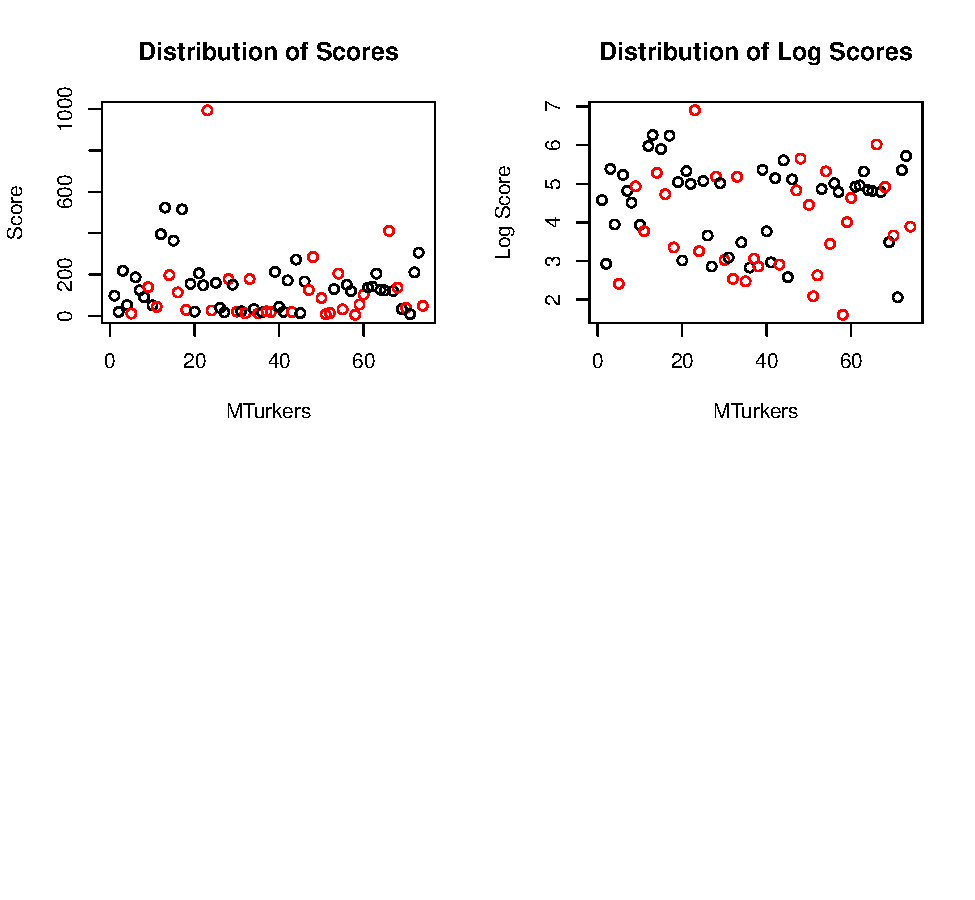
\includegraphics{team_mturk_experiments_files/figure-latex/plot_experiment_1-1.pdf}

\begin{tabular}{l|l}
\hline
  & mean\_worker\_score\\
\hline
 & Min.   :  5.003\\
\hline
 & 1st Qu.: 25.938\\
\hline
 & Median :119.894\\
\hline
 & Mean   :135.288\\
\hline
 & 3rd Qu.:178.160\\
\hline
 & Max.   :994.601\\
\hline
 & NA's   :1\\
\hline
\end{tabular}

\begin{tabular}{r|r|r}
\hline
in\_treatment & mean\_score & std\_dev\\
\hline
0 & 146.7838 & 125.4300\\
\hline
1 & 118.8101 & 190.9985\\
\hline
\end{tabular}

\begin{Shaded}
\begin{Highlighting}[]
\CommentTok{#TODO Gauge if effort decreases with more HITTs}
\end{Highlighting}
\end{Shaded}

\hypertarget{experiment-2-our-second-pilot}{%
\subsubsection{Experiment 2, our second
pilot}\label{experiment-2-our-second-pilot}}

With the first pilot behind us, we decided we needed to focus on
increasing our statistical power and hypothesized that having more
subjects with fewer experiments would provide more statistical power.

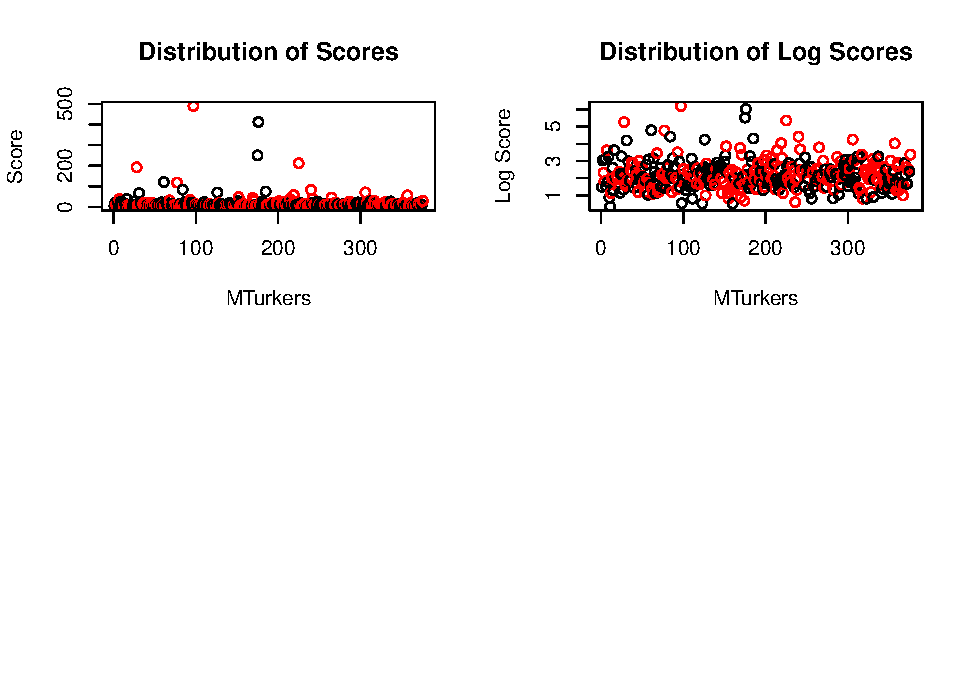
\includegraphics{team_mturk_experiments_files/figure-latex/plot_experiment_2-1.pdf}

\begin{tabular}{l|l}
\hline
  & bounding\_box\_score\\
\hline
 & Min.   :  1.423\\
\hline
 & 1st Qu.:  5.054\\
\hline
 & Median :  8.320\\
\hline
 & Mean   : 16.178\\
\hline
 & 3rd Qu.: 13.498\\
\hline
 & Max.   :489.540\\
\hline
 & NA's   :3\\
\hline
\end{tabular}

\begin{tabular}{r|r|r}
\hline
in\_treatment & mean\_score & std\_dev\\
\hline
0 & 15.25847 & 36.79851\\
\hline
1 & 17.09362 & 42.27343\\
\hline
\end{tabular}

Even with a p-value of 0.655, this was progress. Our coefficient for in
treatment was still more likely due to random noise than not.

\hypertarget{power-test}{%
\paragraph{2.1 Power Test}\label{power-test}}

\begin{verbatim}
## 
##      Two-sample t test power calculation 
## 
##               n = 5756.986
##           delta = 1.835148
##              sd = 39.59534
##       sig.level = 0.05
##           power = 0.8
##     alternative = one.sided
## 
## NOTE: n is number in *each* group
\end{verbatim}

To achieve the statistical power of 0.8 at the 0.05 confidence-level
with the variance we had in this experiement, we would require nearly
5,800 subjects in both control and treatment.

\hypertarget{analysis}{%
\paragraph{2.2 Analysis}\label{analysis}}

With this pilot, the only covariate we had was the amount of time each
Turker spent on the task. And working time acts as a control explaining
away some of the variance reducing the p-value for our target feature
from 0.45 to 0.39.

\begin{Shaded}
\begin{Highlighting}[]
\NormalTok{e2_mod_}\DecValTok{1}\NormalTok{ <-}\StringTok{ }\NormalTok{d[experiment_no}\OperatorTok{==}\DecValTok{2}\NormalTok{, }\KeywordTok{lm}\NormalTok{(bounding_box_score }\OperatorTok{~}\StringTok{ }\NormalTok{in_treatment)]}
\NormalTok{e2_mod_}\DecValTok{2}\NormalTok{ <-}\StringTok{ }\NormalTok{d[experiment_no}\OperatorTok{==}\DecValTok{2}\NormalTok{, }\KeywordTok{lm}\NormalTok{(bounding_box_score }\OperatorTok{~}\StringTok{ }\NormalTok{in_treatment}\OperatorTok{+}\NormalTok{WorkTimeInSeconds)]}

\KeywordTok{stargazer}\NormalTok{(e2_mod_}\DecValTok{1}\NormalTok{,  e2_mod_}\DecValTok{2}\NormalTok{,}
          \DataTypeTok{type =} \StringTok{'latex'}\NormalTok{, }\DataTypeTok{header =} \OtherTok{FALSE}\NormalTok{, }\DataTypeTok{table.placement =} \StringTok{'h'}\NormalTok{, }\DataTypeTok{report=}\NormalTok{(}\StringTok{'vc*p'}\NormalTok{),}
          \DataTypeTok{add.lines =} \KeywordTok{list}\NormalTok{(}\KeywordTok{c}\NormalTok{(}\StringTok{"Data Subset"}\NormalTok{, }\StringTok{"All"}\NormalTok{, }\StringTok{"All"}\NormalTok{, }\StringTok{"$x==1$"}\NormalTok{)),}
          \DataTypeTok{column.labels=}\KeywordTok{c}\NormalTok{(}\StringTok{"Target Alone"}\NormalTok{, }\StringTok{"With WorkInSeconds Control"}\NormalTok{))}
\end{Highlighting}
\end{Shaded}

\begin{table}[h] \centering 
  \caption{} 
  \label{} 
\begin{tabular}{@{\extracolsep{5pt}}lcc} 
\\[-1.8ex]\hline 
\hline \\[-1.8ex] 
 & \multicolumn{2}{c}{\textit{Dependent variable:}} \\ 
\cline{2-3} 
\\[-1.8ex] & \multicolumn{2}{c}{bounding\_box\_score} \\ 
 & Target Alone & With WorkInSeconds Control \\ 
\\[-1.8ex] & (1) & (2)\\ 
\hline \\[-1.8ex] 
 in\_treatment & 1.835 & 1.903 \\ 
  & p = 0.656 & p = 0.644 \\ 
  & & \\ 
 WorkTimeInSeconds &  & 0.010 \\ 
  &  & p = 0.426 \\ 
  & & \\ 
 Constant & 15.258$^{***}$ & 14.441$^{***}$ \\ 
  & p = 0.00000 & p = 0.00001 \\ 
  & & \\ 
\hline \\[-1.8ex] 
Data Subset & All & All \\ 
Observations & 373 & 373 \\ 
R$^{2}$ & 0.001 & 0.002 \\ 
Adjusted R$^{2}$ & $-$0.002 & $-$0.003 \\ 
Residual Std. Error & 39.638 (df = 371) & 39.657 (df = 370) \\ 
F Statistic & 0.200 (df = 1; 371) & 0.418 (df = 2; 370) \\ 
\hline 
\hline \\[-1.8ex] 
\textit{Note:}  & \multicolumn{2}{r}{$^{*}$p$<$0.1; $^{**}$p$<$0.05; $^{***}$p$<$0.01} \\ 
\end{tabular} 
\end{table}

=============================================== Dependent variable:\\
--------------------------- WorkTimeInSeconds\\
----------------------------------------------- in\_treatment -7.720\\
p = 0.663

Constant 86.059***\\
p = 0.000

\begin{longtable}[]{@{}l@{}}
\toprule
\endhead
\begin{minipage}[t]{0.65\columnwidth}\raggedright
Data Subset All Observations 376 R2 0.001 Adjusted R2 -0.002 Residual
Std. Error 171.347 (df = 374) F Statistic 0.191 (df = 1; 374)
=============================================== Note:
\emph{p\textless0.1; \textbf{p\textless0.05; }}p\textless0.01\strut
\end{minipage}\tabularnewline
\begin{minipage}[t]{0.65\columnwidth}\raggedright
The results suggest the negative treatment caused Turkers to spend less
time on the task, but the p-value is far from statistically significant
again.\strut
\end{minipage}\tabularnewline
\begin{minipage}[t]{0.65\columnwidth}\raggedright
\#\#\#\# 2.3 Learnings from our second experiment.\strut
\end{minipage}\tabularnewline
\begin{minipage}[t]{0.65\columnwidth}\raggedright
The estimated 11,600 subjects required to achieve the statistical power
we needed was far too many, With a p-value of 0.389, even with the
11,600 subjects, we weren't likely to find a statistically significant
ATE. We need to change our experiment and collect more covariates.\strut
\end{minipage}\tabularnewline
\begin{minipage}[t]{0.65\columnwidth}\raggedright
\#\#\# Experiment 3, incentive of future work.\strut
\end{minipage}\tabularnewline
\begin{minipage}[t]{0.65\columnwidth}\raggedright
In both of our pilots, we used a treatment which we hypothesized would
cause the Turkers in treatment to work less hard, and the ATE was
positive, which in our scoring means the bounding was less accurate. We
also wanted to test if a positive treatment would have a larger ATE, so
the Turkers in treatment were told we were looking for Turkers to
perform some future work with the hypothesis that if the Turkers though
of the task as a test with the incentive of future work they would try
harder. So we ran a small experiment to test this theory.\strut
\end{minipage}\tabularnewline
\begin{minipage}[t]{0.65\columnwidth}\raggedright
\#\#\#\# 3.1 Simple regression analysis\strut
\end{minipage}\tabularnewline
\begin{minipage}[t]{0.65\columnwidth}\raggedright
```r e3\_mod\_1 \textless- d{[}experiment\_no==3,
lm(bounding\_box\_score \textasciitilde{} in\_treatment){]}\strut
\end{minipage}\tabularnewline
\begin{minipage}[t]{0.65\columnwidth}\raggedright
stargazer(e3\_mod\_1, e2\_mod\_1, type = `text', header = FALSE,
table.placement = `h', report=('vc*p'), add.lines = list(c(``Data
Subset'', ``All'', ``All'', ``\(x==1\)'')),
column.labels=c(``Incentivized'', ``Negative Treatment'')) ```\strut
\end{minipage}\tabularnewline
\begin{minipage}[t]{0.65\columnwidth}\raggedright
\texttt{\#\#\ \#\#\ ==========================================================\ \#\#\ \ \ \ \ \ \ \ \ \ \ \ \ \ \ \ \ \ \ \ \ \ \ \ \ \ \ \ \ \ Dependent\ variable:\ \#\#\ \ \ \ \ \ \ \ \ \ \ \ \ \ \ \ \ \ \ \ \ -\/-\/-\/-\/-\/-\/-\/-\/-\/-\/-\/-\/-\/-\/-\/-\/-\/-\/-\/-\/-\/-\/-\/-\/-\/-\/-\/-\/-\/-\/-\/-\/-\/-\/-\/-\/-\/-\ \#\#\ \ \ \ \ \ \ \ \ \ \ \ \ \ \ \ \ \ \ \ \ \ \ \ \ \ \ \ \ \ \ bounding\_box\_score\ \#\#\ \ \ \ \ \ \ \ \ \ \ \ \ \ \ \ \ \ \ \ \ \ \ \ Incentivized\ \ \ \ Negative\ Treatment\ \#\#\ \ \ \ \ \ \ \ \ \ \ \ \ \ \ \ \ \ \ \ \ \ \ \ \ \ \ \ (1)\ \ \ \ \ \ \ \ \ \ \ \ \ \ \ \ \ (2)\ \#\#\ -\/-\/-\/-\/-\/-\/-\/-\/-\/-\/-\/-\/-\/-\/-\/-\/-\/-\/-\/-\/-\/-\/-\/-\/-\/-\/-\/-\/-\/-\/-\/-\/-\/-\/-\/-\/-\/-\/-\/-\/-\/-\/-\/-\/-\/-\/-\/-\/-\/-\/-\/-\/-\/-\/-\/-\/-\/-\ \#\#\ in\_treatment\ \ \ \ \ \ \ \ \ \ \ \ \ \ 3.687\ \ \ \ \ \ \ \ \ \ \ \ \ \ \ 1.835\ \#\#\ \ \ \ \ \ \ \ \ \ \ \ \ \ \ \ \ \ \ \ \ \ \ \ \ p\ =\ 0.563\ \ \ \ \ \ \ \ \ \ \ p\ =\ 0.656\ \#\#\ \#\#\ Constant\ \ \ \ \ \ \ \ \ \ \ \ \ \ \ \ 19.028***\ \ \ \ \ \ \ \ \ \ \ 15.258***\ \#\#\ \ \ \ \ \ \ \ \ \ \ \ \ \ \ \ \ \ \ \ \ \ \ \ p\ =\ 0.00004\ \ \ \ \ \ \ \ \ p\ =\ 0.00000\ \#\#\ \#\#\ -\/-\/-\/-\/-\/-\/-\/-\/-\/-\/-\/-\/-\/-\/-\/-\/-\/-\/-\/-\/-\/-\/-\/-\/-\/-\/-\/-\/-\/-\/-\/-\/-\/-\/-\/-\/-\/-\/-\/-\/-\/-\/-\/-\/-\/-\/-\/-\/-\/-\/-\/-\/-\/-\/-\/-\/-\/-\ \#\#\ Data\ Subset\ \ \ \ \ \ \ \ \ \ \ \ \ \ \ \ All\ \ \ \ \ \ \ \ \ \ \ \ \ \ \ \ \ All\ \#\#\ Observations\ \ \ \ \ \ \ \ \ \ \ \ \ \ \ \ 92\ \ \ \ \ \ \ \ \ \ \ \ \ \ \ \ \ 373\ \#\#\ R2\ \ \ \ \ \ \ \ \ \ \ \ \ \ \ \ \ \ \ \ \ \ \ \ 0.004\ \ \ \ \ \ \ \ \ \ \ \ \ \ \ 0.001\ \#\#\ Adjusted\ R2\ \ \ \ \ \ \ \ \ \ \ \ \ \ \ -0.007\ \ \ \ \ \ \ \ \ \ \ \ \ -0.002\ \#\#\ Residual\ Std.\ Error\ \ 30.379\ (df\ =\ 90)\ \ \ 39.638\ (df\ =\ 371)\ \#\#\ F\ Statistic\ \ \ \ \ \ \ \ \ 0.338\ (df\ =\ 1;\ 90)\ 0.200\ (df\ =\ 1;\ 371)\ \#\#\ ==========================================================\ \#\#\ Note:\ \ \ \ \ \ \ \ \ \ \ \ \ \ \ \ \ \ \ \ \ \ \ \ \ \ *p\textless{}0.1;\ **p\textless{}0.05;\ ***p\textless{}0.01}\strut
\end{minipage}\tabularnewline
\begin{minipage}[t]{0.65\columnwidth}\raggedright
The first look was disappointing, the last p-value had gone up from 0.45
in the previous experiment to 0.563 in this, but we only used a quarter
the number of subjects. More concerning is the change in the treatment
was estimated to change the direction of the coeffecient, and it is
still positive.\strut
\end{minipage}\tabularnewline
\begin{minipage}[t]{0.65\columnwidth}\raggedright
\#\#\#\# 3.2 Analysis with covariates\strut
\end{minipage}\tabularnewline
\begin{minipage}[t]{0.65\columnwidth}\raggedright
In this experiment we asked the Turkers to answer some questions about
the device they were using, their experience doing these types of tasks
and some demographic info.\strut
\end{minipage}\tabularnewline
\begin{minipage}[t]{0.65\columnwidth}\raggedright
```r e3\_mod\_2 \textless- d{[}experiment\_no==3,
lm(bounding\_box\_score \textasciitilde{}
in\_treatment+as.factor(monitor)){]} e3\_mod\_3 \textless-
d{[}experiment\_no==3, lm(bounding\_box\_score \textasciitilde{}
in\_treatment+as.factor(didbf)){]} e3\_mod\_4 \textless-
d{[}experiment\_no==3, lm(bounding\_box\_score \textasciitilde{}
in\_treatment+as.factor(age)){]} e3\_mod\_5 \textless-
d{[}experiment\_no==3, lm(bounding\_box\_score \textasciitilde{}
in\_treatment+as.factor(edu)){]} e3\_mod\_6 \textless-
d{[}experiment\_no==3, lm(bounding\_box\_score \textasciitilde{}
in\_treatment+as.factor(income)){]}\strut
\end{minipage}\tabularnewline
\begin{minipage}[t]{0.65\columnwidth}\raggedright
stargazer(e3\_mod\_1, e3\_mod\_2, e3\_mod\_3, e3\_mod\_4, e3\_mod\_5,
e3\_mod\_6, type = `text', header = FALSE, table.placement = `h',
report=('vc*p'), add.lines = list(c(``Data Subset'', ``All'', ``All'',
``\(x==1\)'')), column.labels=c(``Target Alone'', ``Monitor size'',
``Did task before'', ``Age'', ``Education'', ``Income'')) ```\strut
\end{minipage}\tabularnewline
\begin{minipage}[t]{0.65\columnwidth}\raggedright
\texttt{\#\#\ \#\#\ =====================================================================================================================================================\ \#\#\ \ \ \ \ \ \ \ \ \ \ \ \ \ \ \ \ \ \ \ \ \ \ \ \ \ \ \ \ \ \ \ \ \ \ \ \ \ \ \ \ \ \ \ \ \ \ \ \ \ \ \ \ \ \ \ \ \ \ \ \ \ \ \ \ \ \ \ \ \ \ \ \ \ \ \ \ \ \ \ \ Dependent\ variable:\ \#\#\ \ \ \ \ \ \ \ \ \ \ \ \ \ \ \ \ \ \ \ \ \ \ \ \ \ \ \ \ \ \ -\/-\/-\/-\/-\/-\/-\/-\/-\/-\/-\/-\/-\/-\/-\/-\/-\/-\/-\/-\/-\/-\/-\/-\/-\/-\/-\/-\/-\/-\/-\/-\/-\/-\/-\/-\/-\/-\/-\/-\/-\/-\/-\/-\/-\/-\/-\/-\/-\/-\/-\/-\/-\/-\/-\/-\/-\/-\/-\/-\/-\/-\/-\/-\/-\/-\/-\/-\/-\/-\/-\/-\/-\/-\/-\/-\/-\/-\/-\/-\/-\/-\/-\/-\/-\/-\/-\/-\/-\/-\/-\/-\/-\/-\/-\/-\/-\/-\/-\/-\/-\/-\/-\/-\/-\/-\/-\/-\/-\/-\/-\/-\/-\/-\/-\/-\/-\/-\/-\ \#\#\ \ \ \ \ \ \ \ \ \ \ \ \ \ \ \ \ \ \ \ \ \ \ \ \ \ \ \ \ \ \ \ \ \ \ \ \ \ \ \ \ \ \ \ \ \ \ \ \ \ \ \ \ \ \ \ \ \ \ \ \ \ \ \ \ \ \ \ \ \ \ \ \ \ \ \ \ \ \ \ \ bounding\_box\_score\ \#\#\ \ \ \ \ \ \ \ \ \ \ \ \ \ \ \ \ \ \ \ \ \ \ \ \ \ \ \ \ \ \ \ \ \ Target\ Alone\ \ \ \ \ \ \ \ Monitor\ size\ \ \ \ \ \ \ Did\ task\ before\ \ \ \ \ \ \ \ \ \ \ \ Age\ \ \ \ \ \ \ \ \ \ \ \ \ \ Education\ \ \ \ \ \ \ \ \ \ \ \ Income\ \#\#\ \ \ \ \ \ \ \ \ \ \ \ \ \ \ \ \ \ \ \ \ \ \ \ \ \ \ \ \ \ \ \ \ \ \ \ \ \ (1)\ \ \ \ \ \ \ \ \ \ \ \ \ \ \ \ \ \ (2)\ \ \ \ \ \ \ \ \ \ \ \ \ \ \ \ \ (3)\ \ \ \ \ \ \ \ \ \ \ \ \ \ \ \ \ \ (4)\ \ \ \ \ \ \ \ \ \ \ \ \ \ \ \ \ (5)\ \ \ \ \ \ \ \ \ \ \ \ \ \ \ \ (6)\ \#\#\ -\/-\/-\/-\/-\/-\/-\/-\/-\/-\/-\/-\/-\/-\/-\/-\/-\/-\/-\/-\/-\/-\/-\/-\/-\/-\/-\/-\/-\/-\/-\/-\/-\/-\/-\/-\/-\/-\/-\/-\/-\/-\/-\/-\/-\/-\/-\/-\/-\/-\/-\/-\/-\/-\/-\/-\/-\/-\/-\/-\/-\/-\/-\/-\/-\/-\/-\/-\/-\/-\/-\/-\/-\/-\/-\/-\/-\/-\/-\/-\/-\/-\/-\/-\/-\/-\/-\/-\/-\/-\/-\/-\/-\/-\/-\/-\/-\/-\/-\/-\/-\/-\/-\/-\/-\/-\/-\/-\/-\/-\/-\/-\/-\/-\/-\/-\/-\/-\/-\/-\/-\/-\/-\/-\/-\/-\/-\/-\/-\/-\/-\/-\/-\/-\/-\/-\/-\/-\/-\/-\/-\/-\/-\/-\/-\/-\/-\/-\/-\ \#\#\ in\_treatment\ \ \ \ \ \ \ \ \ \ \ \ \ \ \ \ \ \ \ \ \ \ \ \ 3.687\ \ \ \ \ \ \ \ \ \ \ \ \ \ \ \ 7.794\ \ \ \ \ \ \ \ \ \ \ \ \ \ \ 4.708\ \ \ \ \ \ \ \ \ \ \ \ \ \ \ \ 2.681\ \ \ \ \ \ \ \ \ \ \ \ \ \ \ 3.280\ \ \ \ \ \ \ \ \ \ \ \ \ \ -0.015\ \#\#\ \ \ \ \ \ \ \ \ \ \ \ \ \ \ \ \ \ \ \ \ \ \ \ \ \ \ \ \ \ \ \ \ \ \ p\ =\ 0.563\ \ \ \ \ \ \ \ \ \ \ \ p\ =\ 0.231\ \ \ \ \ \ \ \ \ \ \ p\ =\ 0.470\ \ \ \ \ \ \ \ \ \ \ \ p\ =\ 0.640\ \ \ \ \ \ \ \ \ \ \ p\ =\ 0.613\ \ \ \ \ \ \ \ \ \ p\ =\ 0.999\ \#\#\ \#\#\ as.factor(monitor)largescreen\ \ \ \ \ \ \ \ \ \ \ \ \ \ \ \ \ \ \ \ \ \ \ \ \ -66.462***\ \#\#\ \ \ \ \ \ \ \ \ \ \ \ \ \ \ \ \ \ \ \ \ \ \ \ \ \ \ \ \ \ \ \ \ \ \ \ \ \ \ \ \ \ \ \ \ \ \ \ \ \ \ \ \ \ \ p\ =\ 0.0004\ \#\#\ \#\#\ as.factor(monitor)midsize\ \ \ \ \ \ \ \ \ \ \ \ \ \ \ \ \ \ \ \ \ \ \ \ \ \ \ \ \ -60.451***\ \#\#\ \ \ \ \ \ \ \ \ \ \ \ \ \ \ \ \ \ \ \ \ \ \ \ \ \ \ \ \ \ \ \ \ \ \ \ \ \ \ \ \ \ \ \ \ \ \ \ \ \ \ \ \ \ \ p\ =\ 0.0005\ \#\#\ \#\#\ as.factor(monitor)smalllaptop\ \ \ \ \ \ \ \ \ \ \ \ \ \ \ \ \ \ \ \ \ \ \ \ \ -57.383***\ \#\#\ \ \ \ \ \ \ \ \ \ \ \ \ \ \ \ \ \ \ \ \ \ \ \ \ \ \ \ \ \ \ \ \ \ \ \ \ \ \ \ \ \ \ \ \ \ \ \ \ \ \ \ \ \ \ \ p\ =\ 0.002\ \#\#\ \#\#\ as.factor(monitor)tablet\ \ \ \ \ \ \ \ \ \ \ \ \ \ \ \ \ \ \ \ \ \ \ \ \ \ \ \ \ \ \ -35.061*\ \#\#\ \ \ \ \ \ \ \ \ \ \ \ \ \ \ \ \ \ \ \ \ \ \ \ \ \ \ \ \ \ \ \ \ \ \ \ \ \ \ \ \ \ \ \ \ \ \ \ \ \ \ \ \ \ \ \ p\ =\ 0.064\ \#\#\ \#\#\ as.factor(didbf)no\ \ \ \ \ \ \ \ \ \ \ \ \ \ \ \ \ \ \ \ \ \ \ \ \ \ \ \ \ \ \ \ \ \ \ \ \ \ \ \ \ \ \ \ \ \ \ \ \ \ \ \ \ \ \ \ \ \ \ 7.732\ \#\#\ \ \ \ \ \ \ \ \ \ \ \ \ \ \ \ \ \ \ \ \ \ \ \ \ \ \ \ \ \ \ \ \ \ \ \ \ \ \ \ \ \ \ \ \ \ \ \ \ \ \ \ \ \ \ \ \ \ \ \ \ \ \ \ \ \ \ \ \ \ \ \ \ \ \ \ p\ =\ 0.612\ \#\#\ \#\#\ as.factor(didbf)yes\ \ \ \ \ \ \ \ \ \ \ \ \ \ \ \ \ \ \ \ \ \ \ \ \ \ \ \ \ \ \ \ \ \ \ \ \ \ \ \ \ \ \ \ \ \ \ \ \ \ \ \ \ \ \ \ \ \ 8.810\ \#\#\ \ \ \ \ \ \ \ \ \ \ \ \ \ \ \ \ \ \ \ \ \ \ \ \ \ \ \ \ \ \ \ \ \ \ \ \ \ \ \ \ \ \ \ \ \ \ \ \ \ \ \ \ \ \ \ \ \ \ \ \ \ \ \ \ \ \ \ \ \ \ \ \ \ \ \ p\ =\ 0.535\ \#\#\ \#\#\ as.factor(age)31to40\ \ \ \ \ \ \ \ \ \ \ \ \ \ \ \ \ \ \ \ \ \ \ \ \ \ \ \ \ \ \ \ \ \ \ \ \ \ \ \ \ \ \ \ \ \ \ \ \ \ \ \ \ \ \ \ \ \ \ \ \ \ \ \ \ \ \ \ \ \ \ \ \ \ \ \ \ -9.611\ \#\#\ \ \ \ \ \ \ \ \ \ \ \ \ \ \ \ \ \ \ \ \ \ \ \ \ \ \ \ \ \ \ \ \ \ \ \ \ \ \ \ \ \ \ \ \ \ \ \ \ \ \ \ \ \ \ \ \ \ \ \ \ \ \ \ \ \ \ \ \ \ \ \ \ \ \ \ \ \ \ \ \ \ \ \ \ \ \ \ \ \ \ \ \ \ \ \ \ p\ =\ 0.372\ \#\#\ \#\#\ as.factor(age)41to50\ \ \ \ \ \ \ \ \ \ \ \ \ \ \ \ \ \ \ \ \ \ \ \ \ \ \ \ \ \ \ \ \ \ \ \ \ \ \ \ \ \ \ \ \ \ \ \ \ \ \ \ \ \ \ \ \ \ \ \ \ \ \ \ \ \ \ \ \ \ \ \ \ \ \ \ 97.704***\ \#\#\ \ \ \ \ \ \ \ \ \ \ \ \ \ \ \ \ \ \ \ \ \ \ \ \ \ \ \ \ \ \ \ \ \ \ \ \ \ \ \ \ \ \ \ \ \ \ \ \ \ \ \ \ \ \ \ \ \ \ \ \ \ \ \ \ \ \ \ \ \ \ \ \ \ \ \ \ \ \ \ \ \ \ \ \ \ \ \ \ \ \ \ \ \ \ \ p\ =\ 0.00001\ \#\#\ \#\#\ as.factor(age)lt21\ \ \ \ \ \ \ \ \ \ \ \ \ \ \ \ \ \ \ \ \ \ \ \ \ \ \ \ \ \ \ \ \ \ \ \ \ \ \ \ \ \ \ \ \ \ \ \ \ \ \ \ \ \ \ \ \ \ \ \ \ \ \ \ \ \ \ \ \ \ \ \ \ \ \ \ \ \ \ -12.327\ \#\#\ \ \ \ \ \ \ \ \ \ \ \ \ \ \ \ \ \ \ \ \ \ \ \ \ \ \ \ \ \ \ \ \ \ \ \ \ \ \ \ \ \ \ \ \ \ \ \ \ \ \ \ \ \ \ \ \ \ \ \ \ \ \ \ \ \ \ \ \ \ \ \ \ \ \ \ \ \ \ \ \ \ \ \ \ \ \ \ \ \ \ \ \ \ \ \ \ p\ =\ 0.653\ \#\#\ \#\#\ as.factor(edu)highschool\ \ \ \ \ \ \ \ \ \ \ \ \ \ \ \ \ \ \ \ \ \ \ \ \ \ \ \ \ \ \ \ \ \ \ \ \ \ \ \ \ \ \ \ \ \ \ \ \ \ \ \ \ \ \ \ \ \ \ \ \ \ \ \ \ \ \ \ \ \ \ \ \ \ \ \ \ \ \ \ \ \ \ \ \ \ \ \ \ \ \ \ \ -17.099\ \#\#\ \ \ \ \ \ \ \ \ \ \ \ \ \ \ \ \ \ \ \ \ \ \ \ \ \ \ \ \ \ \ \ \ \ \ \ \ \ \ \ \ \ \ \ \ \ \ \ \ \ \ \ \ \ \ \ \ \ \ \ \ \ \ \ \ \ \ \ \ \ \ \ \ \ \ \ \ \ \ \ \ \ \ \ \ \ \ \ \ \ \ \ \ \ \ \ \ \ \ \ \ \ \ \ \ \ \ \ \ \ \ \ \ \ \ \ \ p\ =\ 0.438\ \#\#\ \#\#\ as.factor(edu)masterorabove\ \ \ \ \ \ \ \ \ \ \ \ \ \ \ \ \ \ \ \ \ \ \ \ \ \ \ \ \ \ \ \ \ \ \ \ \ \ \ \ \ \ \ \ \ \ \ \ \ \ \ \ \ \ \ \ \ \ \ \ \ \ \ \ \ \ \ \ \ \ \ \ \ \ \ \ \ \ \ \ \ \ \ \ \ \ \ \ \ \ -14.161\ \#\#\ \ \ \ \ \ \ \ \ \ \ \ \ \ \ \ \ \ \ \ \ \ \ \ \ \ \ \ \ \ \ \ \ \ \ \ \ \ \ \ \ \ \ \ \ \ \ \ \ \ \ \ \ \ \ \ \ \ \ \ \ \ \ \ \ \ \ \ \ \ \ \ \ \ \ \ \ \ \ \ \ \ \ \ \ \ \ \ \ \ \ \ \ \ \ \ \ \ \ \ \ \ \ \ \ \ \ \ \ \ \ \ \ \ \ \ \ p\ =\ 0.154\ \#\#\ \#\#\ as.factor(edu)somecollege\ \ \ \ \ \ \ \ \ \ \ \ \ \ \ \ \ \ \ \ \ \ \ \ \ \ \ \ \ \ \ \ \ \ \ \ \ \ \ \ \ \ \ \ \ \ \ \ \ \ \ \ \ \ \ \ \ \ \ \ \ \ \ \ \ \ \ \ \ \ \ \ \ \ \ \ \ \ \ \ \ \ \ \ \ \ \ \ \ \ \ \ -15.051\ \#\#\ \ \ \ \ \ \ \ \ \ \ \ \ \ \ \ \ \ \ \ \ \ \ \ \ \ \ \ \ \ \ \ \ \ \ \ \ \ \ \ \ \ \ \ \ \ \ \ \ \ \ \ \ \ \ \ \ \ \ \ \ \ \ \ \ \ \ \ \ \ \ \ \ \ \ \ \ \ \ \ \ \ \ \ \ \ \ \ \ \ \ \ \ \ \ \ \ \ \ \ \ \ \ \ \ \ \ \ \ \ \ \ \ \ \ \ \ p\ =\ 0.216\ \#\#\ \#\#\ as.factor(income)gt30klt60k\ \ \ \ \ \ \ \ \ \ \ \ \ \ \ \ \ \ \ \ \ \ \ \ \ \ \ \ \ \ \ \ \ \ \ \ \ \ \ \ \ \ \ \ \ \ \ \ \ \ \ \ \ \ \ \ \ \ \ \ \ \ \ \ \ \ \ \ \ \ \ \ \ \ \ \ \ \ \ \ \ \ \ \ \ \ \ \ \ \ \ \ \ \ \ \ \ \ \ \ \ \ \ \ \ \ \ \ \ \ 7.338\ \#\#\ \ \ \ \ \ \ \ \ \ \ \ \ \ \ \ \ \ \ \ \ \ \ \ \ \ \ \ \ \ \ \ \ \ \ \ \ \ \ \ \ \ \ \ \ \ \ \ \ \ \ \ \ \ \ \ \ \ \ \ \ \ \ \ \ \ \ \ \ \ \ \ \ \ \ \ \ \ \ \ \ \ \ \ \ \ \ \ \ \ \ \ \ \ \ \ \ \ \ \ \ \ \ \ \ \ \ \ \ \ \ \ \ \ \ \ \ \ \ \ \ \ \ \ \ \ \ \ \ \ \ \ \ \ \ \ p\ =\ 0.371\ \#\#\ \#\#\ as.factor(income)gt60klt90k\ \ \ \ \ \ \ \ \ \ \ \ \ \ \ \ \ \ \ \ \ \ \ \ \ \ \ \ \ \ \ \ \ \ \ \ \ \ \ \ \ \ \ \ \ \ \ \ \ \ \ \ \ \ \ \ \ \ \ \ \ \ \ \ \ \ \ \ \ \ \ \ \ \ \ \ \ \ \ \ \ \ \ \ \ \ \ \ \ \ \ \ \ \ \ \ \ \ \ \ \ \ \ \ \ \ \ \ \ \ -3.268\ \#\#\ \ \ \ \ \ \ \ \ \ \ \ \ \ \ \ \ \ \ \ \ \ \ \ \ \ \ \ \ \ \ \ \ \ \ \ \ \ \ \ \ \ \ \ \ \ \ \ \ \ \ \ \ \ \ \ \ \ \ \ \ \ \ \ \ \ \ \ \ \ \ \ \ \ \ \ \ \ \ \ \ \ \ \ \ \ \ \ \ \ \ \ \ \ \ \ \ \ \ \ \ \ \ \ \ \ \ \ \ \ \ \ \ \ \ \ \ \ \ \ \ \ \ \ \ \ \ \ \ \ \ \ \ \ \ \ p\ =\ 0.762\ \#\#\ \#\#\ as.factor(income)gt90k\ \ \ \ \ \ \ \ \ \ \ \ \ \ \ \ \ \ \ \ \ \ \ \ \ \ \ \ \ \ \ \ \ \ \ \ \ \ \ \ \ \ \ \ \ \ \ \ \ \ \ \ \ \ \ \ \ \ \ \ \ \ \ \ \ \ \ \ \ \ \ \ \ \ \ \ \ \ \ \ \ \ \ \ \ \ \ \ \ \ \ \ \ \ \ \ \ \ \ \ \ \ \ \ \ \ \ \ \ \ \ \ \ \ \ 19.021\ \#\#\ \ \ \ \ \ \ \ \ \ \ \ \ \ \ \ \ \ \ \ \ \ \ \ \ \ \ \ \ \ \ \ \ \ \ \ \ \ \ \ \ \ \ \ \ \ \ \ \ \ \ \ \ \ \ \ \ \ \ \ \ \ \ \ \ \ \ \ \ \ \ \ \ \ \ \ \ \ \ \ \ \ \ \ \ \ \ \ \ \ \ \ \ \ \ \ \ \ \ \ \ \ \ \ \ \ \ \ \ \ \ \ \ \ \ \ \ \ \ \ \ \ \ \ \ \ \ \ \ \ \ \ \ \ \ \ p\ =\ 0.160\ \#\#\ \#\#\ as.factor(income)lt10k\ \ \ \ \ \ \ \ \ \ \ \ \ \ \ \ \ \ \ \ \ \ \ \ \ \ \ \ \ \ \ \ \ \ \ \ \ \ \ \ \ \ \ \ \ \ \ \ \ \ \ \ \ \ \ \ \ \ \ \ \ \ \ \ \ \ \ \ \ \ \ \ \ \ \ \ \ \ \ \ \ \ \ \ \ \ \ \ \ \ \ \ \ \ \ \ \ \ \ \ \ \ \ \ \ \ \ \ \ \ \ \ \ \ \ -8.956\ \#\#\ \ \ \ \ \ \ \ \ \ \ \ \ \ \ \ \ \ \ \ \ \ \ \ \ \ \ \ \ \ \ \ \ \ \ \ \ \ \ \ \ \ \ \ \ \ \ \ \ \ \ \ \ \ \ \ \ \ \ \ \ \ \ \ \ \ \ \ \ \ \ \ \ \ \ \ \ \ \ \ \ \ \ \ \ \ \ \ \ \ \ \ \ \ \ \ \ \ \ \ \ \ \ \ \ \ \ \ \ \ \ \ \ \ \ \ \ \ \ \ \ \ \ \ \ \ \ \ \ \ \ \ \ \ \ \ p\ =\ 0.404\ \#\#\ \#\#\ Constant\ \ \ \ \ \ \ \ \ \ \ \ \ \ \ \ \ \ \ \ \ \ \ \ \ \ 19.028***\ \ \ \ \ \ \ \ \ \ \ \ 72.889***\ \ \ \ \ \ \ \ \ \ \ \ \ 9.539\ \ \ \ \ \ \ \ \ \ \ \ \ \ 18.250***\ \ \ \ \ \ \ \ \ \ \ 22.433***\ \ \ \ \ \ \ \ \ \ 18.375***\ \#\#\ \ \ \ \ \ \ \ \ \ \ \ \ \ \ \ \ \ \ \ \ \ \ \ \ \ \ \ \ \ \ \ \ \ p\ =\ 0.00004\ \ \ \ \ \ \ \ \ \ p\ =\ 0.00004\ \ \ \ \ \ \ \ \ \ p\ =\ 0.474\ \ \ \ \ \ \ \ \ \ \ p\ =\ 0.00003\ \ \ \ \ \ \ \ \ p\ =\ 0.00001\ \ \ \ \ \ \ \ \ p\ =\ 0.002\ \#\#\ \#\#\ -\/-\/-\/-\/-\/-\/-\/-\/-\/-\/-\/-\/-\/-\/-\/-\/-\/-\/-\/-\/-\/-\/-\/-\/-\/-\/-\/-\/-\/-\/-\/-\/-\/-\/-\/-\/-\/-\/-\/-\/-\/-\/-\/-\/-\/-\/-\/-\/-\/-\/-\/-\/-\/-\/-\/-\/-\/-\/-\/-\/-\/-\/-\/-\/-\/-\/-\/-\/-\/-\/-\/-\/-\/-\/-\/-\/-\/-\/-\/-\/-\/-\/-\/-\/-\/-\/-\/-\/-\/-\/-\/-\/-\/-\/-\/-\/-\/-\/-\/-\/-\/-\/-\/-\/-\/-\/-\/-\/-\/-\/-\/-\/-\/-\/-\/-\/-\/-\/-\/-\/-\/-\/-\/-\/-\/-\/-\/-\/-\/-\/-\/-\/-\/-\/-\/-\/-\/-\/-\/-\/-\/-\/-\/-\/-\/-\/-\/-\/-\ \#\#\ Data\ Subset\ \ \ \ \ \ \ \ \ \ \ \ \ \ \ \ \ \ \ \ \ \ \ \ \ \ All\ \ \ \ \ \ \ \ \ \ \ \ \ \ \ \ \ \ All\ \ \ \ \ \ \ \ \ \ \ \ \ \ \ \ \ x==1\ \#\#\ Observations\ \ \ \ \ \ \ \ \ \ \ \ \ \ \ \ \ \ \ \ \ \ \ \ \ \ 92\ \ \ \ \ \ \ \ \ \ \ \ \ \ \ \ \ \ 92\ \ \ \ \ \ \ \ \ \ \ \ \ \ \ \ \ \ \ 90\ \ \ \ \ \ \ \ \ \ \ \ \ \ \ \ \ \ 92\ \ \ \ \ \ \ \ \ \ \ \ \ \ \ \ \ \ \ 92\ \ \ \ \ \ \ \ \ \ \ \ \ \ \ \ \ 92\ \#\#\ R2\ \ \ \ \ \ \ \ \ \ \ \ \ \ \ \ \ \ \ \ \ \ \ \ \ \ \ \ \ \ \ \ \ \ 0.004\ \ \ \ \ \ \ \ \ \ \ \ \ \ \ \ 0.200\ \ \ \ \ \ \ \ \ \ \ \ \ \ \ 0.014\ \ \ \ \ \ \ \ \ \ \ \ \ \ \ \ 0.240\ \ \ \ \ \ \ \ \ \ \ \ \ \ \ 0.045\ \ \ \ \ \ \ \ \ \ \ \ \ \ 0.056\ \#\#\ Adjusted\ R2\ \ \ \ \ \ \ \ \ \ \ \ \ \ \ \ \ \ \ \ \ \ \ \ \ -0.007\ \ \ \ \ \ \ \ \ \ \ \ \ \ \ 0.153\ \ \ \ \ \ \ \ \ \ \ \ \ \ \ -0.021\ \ \ \ \ \ \ \ \ \ \ \ \ \ \ 0.205\ \ \ \ \ \ \ \ \ \ \ \ \ \ \ 0.001\ \ \ \ \ \ \ \ \ \ \ \ \ \ 0.001\ \#\#\ Residual\ Std.\ Error\ \ \ \ \ \ \ \ \ \ \ \ 30.379\ (df\ =\ 90)\ \ \ \ 27.850\ (df\ =\ 86)\ \ \ \ \ 29.643\ (df\ =\ 86)\ \ \ \ 26.982\ (df\ =\ 87)\ \ \ \ \ 30.255\ (df\ =\ 87)\ \ \ 30.251\ (df\ =\ 86)\ \#\#\ F\ Statistic\ \ \ \ \ \ \ \ \ \ \ \ \ \ \ \ \ \ \ 0.338\ (df\ =\ 1;\ 90)\ 4.297***\ (df\ =\ 5;\ 86)\ 0.393\ (df\ =\ 3;\ 86)\ 6.879***\ (df\ =\ 4;\ 87)\ 1.021\ (df\ =\ 4;\ 87)\ 1.021\ (df\ =\ 5;\ 86)\ \#\#\ =====================================================================================================================================================\ \#\#\ Note:\ \ \ \ \ \ \ \ \ \ \ \ \ \ \ \ \ \ \ \ \ \ \ \ \ \ \ \ \ \ \ \ \ \ \ \ \ \ \ \ \ \ \ \ \ \ \ \ \ \ \ \ \ \ \ \ \ \ \ \ \ \ \ \ \ \ \ \ \ \ \ \ \ \ \ \ \ \ \ \ \ \ \ \ \ \ \ \ \ \ \ \ \ \ \ \ \ \ \ \ \ \ \ \ \ \ \ \ \ \ \ \ \ \ \ \ \ *p\textless{}0.1;\ **p\textless{}0.05;\ ***p\textless{}0.01}\strut
\end{minipage}\tabularnewline
\begin{minipage}[t]{0.65\columnwidth}\raggedright
The only covariate which seemed to act as any type of control was the
education question, though it wasn't very significant. However, all of
the coeffecients for the screensize question were negative, and by a
fairly significant ammount. The baseline value was cellphone, which can
be significantly smaller than all the other types of screens. So we
tested that on its own.\strut
\end{minipage}\tabularnewline
\begin{minipage}[t]{0.65\columnwidth}\raggedright
===============================================================
Dependent variable: ----------------------------------------
bounding\_box\_score Target Alone Used Cellphone (1) (2)\strut
\end{minipage}\tabularnewline
\bottomrule
\end{longtable}

in\_treatment 3.687 2.239\\
p = 0.563 p = 0.710

monitor == ``cellphone'' 58.789***\\
p = 0.001

Constant 19.028*** 17.803***\\
p = 0.00004 p = 0.00005

\begin{longtable}[]{@{}l@{}}
\toprule
\endhead
\begin{minipage}[t]{0.86\columnwidth}\raggedright
Data Subset All All Observations 92 92 R2 0.004 0.123 Adjusted R2 -0.007
0.104 Residual Std. Error 30.379 (df = 90) 28.655 (df = 89) F Statistic
0.338 (df = 1; 90) 6.268*** (df = 2; 89)
=============================================================== Note:
\emph{p\textless0.1; \textbf{p\textless0.05; }}p\textless0.01\strut
\end{minipage}\tabularnewline
\begin{minipage}[t]{0.86\columnwidth}\raggedright
If the subject is using a cellphone to do the task, their accuracy goes
down (score increases), which is intuitive. Having cellphone as a
control decreases the p-value from 0.56 to 0.33. With more data, this
could be quite a bit lower. But it still doesn't explain why subjects
with more incentive are doing a poorer job.\strut
\end{minipage}\tabularnewline
\begin{minipage}[t]{0.86\columnwidth}\raggedright
As with the previous experiment, we also analyzed how the treatment
affected the amount of time they spent on the task.\strut
\end{minipage}\tabularnewline
\begin{minipage}[t]{0.86\columnwidth}\raggedright
========================================================== Dependent
variable: -------------------------------------- WorkTimeInSeconds
Incentivized Negative Treatment (1) (2)\strut
\end{minipage}\tabularnewline
\bottomrule
\end{longtable}

in\_treatment 22.983 -7.720\\
p = 0.766 p = 0.663

Constant 377.208*** 86.059***\\
p = 0.000 p = 0.000

\begin{longtable}[]{@{}l@{}}
\toprule
\endhead
\begin{minipage}[t]{0.79\columnwidth}\raggedright
Data Subset All All Observations 95 376 R2 0.001 0.001 Adjusted R2
-0.010 -0.002 Residual Std. Error 374.924 (df = 93) 171.347 (df = 374) F
Statistic 0.089 (df = 1; 93) 0.191 (df = 1; 374)
========================================================== Note:
\emph{p\textless0.1; \textbf{p\textless0.05; }}p\textless0.01\strut
\end{minipage}\tabularnewline
\begin{minipage}[t]{0.79\columnwidth}\raggedright
The regression shows those in treatment on average spent 23 seconds more
time, this alone is concerning, as the task itself shouldn't take that
much time.\strut
\end{minipage}\tabularnewline
\begin{minipage}[t]{0.79\columnwidth}\raggedright
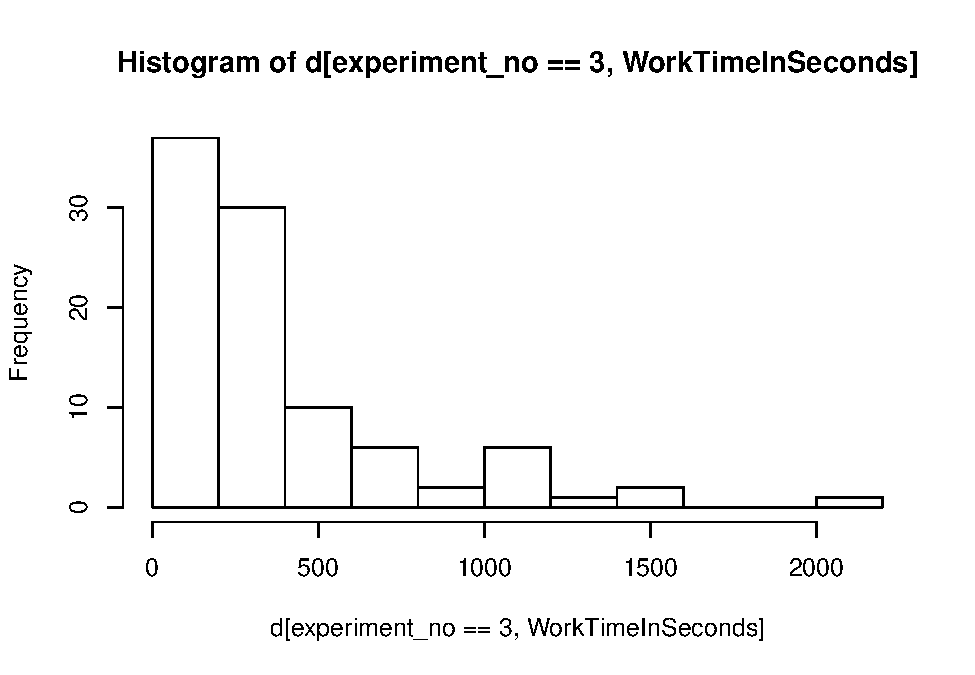
\includegraphics{team_mturk_experiments_files/figure-latex/experiment_3_summary_time-1.pdf}\strut
\end{minipage}\tabularnewline
\begin{minipage}[t]{0.79\columnwidth}\raggedright
There are alot of values suggesting that Turkers are not conentrating on
our task, it could be they are spawning multiple tabs. Regardless,
working time is not helpful for our experiment.\strut
\end{minipage}\tabularnewline
\begin{minipage}[t]{0.79\columnwidth}\raggedright
\#\#\#\# 3.1 Power Test\strut
\end{minipage}\tabularnewline
\begin{minipage}[t]{0.79\columnwidth}\raggedright
With a lot of speculation about whether our statistical significance
would go up with more data, we tested that theory by doing a power
calculation.\strut
\end{minipage}\tabularnewline
\begin{minipage}[t]{0.79\columnwidth}\raggedright
\texttt{\#\#\ \#\#\ \ \ \ \ \ Two-sample\ t\ test\ power\ calculation\ \#\#\ \#\#\ \ \ \ \ \ \ \ \ \ \ \ \ \ \ n\ =\ 834.1739\ \#\#\ \ \ \ \ \ \ \ \ \ \ delta\ =\ 3.686703\ \#\#\ \ \ \ \ \ \ \ \ \ \ \ \ \ sd\ =\ 30.26851\ \#\#\ \ \ \ \ \ \ sig.level\ =\ 0.05\ \#\#\ \ \ \ \ \ \ \ \ \ \ power\ =\ 0.8\ \#\#\ \ \ \ \ alternative\ =\ one.sided\ \#\#\ \#\#\ NOTE:\ n\ is\ number\ in\ *each*\ group}\strut
\end{minipage}\tabularnewline
\begin{minipage}[t]{0.79\columnwidth}\raggedright
The power calculation when using the negative treatment, telling those
in treatment that they were doing work for a government surveillance
system estimated we needed 5,800 subjects. Using an incentive of
possible future work as the treatment, the ATE has less variance, and
estimated that we only need 835 subjects to get 0.80 statistical
power.\strut
\end{minipage}\tabularnewline
\begin{minipage}[t]{0.79\columnwidth}\raggedright
\#\#\# Experiment 4, More data\strut
\end{minipage}\tabularnewline
\begin{minipage}[t]{0.79\columnwidth}\raggedright
To improve the statistical power from Experiment 3, we are adding more
data and sending out another 100 control tasks to Turkers and 100 with
the same treatment.\strut
\end{minipage}\tabularnewline
\begin{minipage}[t]{0.79\columnwidth}\raggedright
\#TODO covariate balance check, demographic info show how random it
is.\strut
\end{minipage}\tabularnewline
\begin{minipage}[t]{0.79\columnwidth}\raggedright
========================================================== Dependent
variable: -------------------------------------- bounding\_box\_score
n=100 + n=200 n=100 (1) (2)\strut
\end{minipage}\tabularnewline
\bottomrule
\end{longtable}

in\_treatment -15.895 3.687\\
p = 0.116 p = 0.563

Constant 33.046*** 19.028***\\
p = 0.00001 p = 0.00004

\begin{longtable}[]{@{}l@{}}
\toprule
\endhead
\begin{minipage}[t]{0.79\columnwidth}\raggedright
Data Subset All All Observations 277 92 R2 0.009 0.004 Adjusted R2 0.005
-0.007 Residual Std. Error 83.748 (df = 275) 30.379 (df = 90) F
Statistic 2.494 (df = 1; 275) 0.338 (df = 1; 90)
========================================================== Note:
\emph{p\textless0.1; \textbf{p\textless0.05; }}p\textless0.01\strut
\end{minipage}\tabularnewline
\begin{minipage}[t]{0.79\columnwidth}\raggedright
The results are much better, adding another 200 subjects helped decrease
the p-value from 0.56 to 0.12, and our ATE is -15.9, a negative number
means the bounding boxes from treatment are more accurate.\strut
\end{minipage}\tabularnewline
\begin{minipage}[t]{0.79\columnwidth}\raggedright
```r \#e4\_mod\_2 \textless- d{[}experiment\_no \%in\% c(3,4),
lm(bounding\_box\_score \textasciitilde{}
in\_treatment+is\_mobile+tried=(monitor=="" \& mousetrackpad=="")){]}
\#summary(e4\_mod\_2)\strut
\end{minipage}\tabularnewline
\begin{minipage}[t]{0.79\columnwidth}\raggedright
\#e4\_mod\_2 \textless- d{[}experiment\_no \%in\% c(3,4),
.(tried=as.numeric(is.na(monitor) \& is.na(mousetrackpad)),
bounding\_box\_score, in\_treatment, is\_mobile, WorkTimeInSeconds){]}
\%\textgreater\% \# .{[}, lm(bounding\_box\_score \textasciitilde{}
in\_treatment+is\_mobile+tried){]} \#summary(e4\_mod\_2)\strut
\end{minipage}\tabularnewline
\begin{minipage}[t]{0.79\columnwidth}\raggedright
\#e4\_mod\_2 \textless- d{[}experiment\_no \%in\% c(3,4),
.(tried=as.numeric(is.na(monitor)), bounding\_box\_score, in\_treatment,
is\_mobile, Reward){]} \%\textgreater\% \# .{[}, lm(bounding\_box\_score
\textasciitilde{} in\_treatment+is\_mobile+tried){]}
\#summary(e4\_mod\_2)\strut
\end{minipage}\tabularnewline
\begin{minipage}[t]{0.79\columnwidth}\raggedright
e4\_mod\_2 \textless- d{[}experiment\_no \%in\% c(3,4),
lm(bounding\_box\_score \textasciitilde{} in\_treatment+is\_mobile){]}
stargazer(e4\_mod\_1, e4\_mod\_2, type = `text', header = FALSE,
table.placement = `h', report=('vc*p'), add.lines = list(c(``Data
Subset'', ``All'', ``All'', ``\(x==1\)'')), column.labels=c(``Target
Alone'', ``Cellphone'')) ```\strut
\end{minipage}\tabularnewline
\begin{minipage}[t]{0.79\columnwidth}\raggedright
\texttt{\#\#\ \#\#\ ==============================================================\ \#\#\ \ \ \ \ \ \ \ \ \ \ \ \ \ \ \ \ \ \ \ \ \ \ \ \ \ \ \ \ \ \ \ Dependent\ variable:\ \#\#\ \ \ \ \ \ \ \ \ \ \ \ \ \ \ \ \ \ \ \ \ -\/-\/-\/-\/-\/-\/-\/-\/-\/-\/-\/-\/-\/-\/-\/-\/-\/-\/-\/-\/-\/-\/-\/-\/-\/-\/-\/-\/-\/-\/-\/-\/-\/-\/-\/-\/-\/-\/-\/-\/-\/-\ \#\#\ \ \ \ \ \ \ \ \ \ \ \ \ \ \ \ \ \ \ \ \ \ \ \ \ \ \ \ \ \ \ \ \ bounding\_box\_score\ \#\#\ \ \ \ \ \ \ \ \ \ \ \ \ \ \ \ \ \ \ \ \ \ \ \ Target\ Alone\ \ \ \ \ \ \ \ \ \ \ Cellphone\ \#\#\ \ \ \ \ \ \ \ \ \ \ \ \ \ \ \ \ \ \ \ \ \ \ \ \ \ \ \ \ (1)\ \ \ \ \ \ \ \ \ \ \ \ \ \ \ \ \ \ (2)\ \#\#\ -\/-\/-\/-\/-\/-\/-\/-\/-\/-\/-\/-\/-\/-\/-\/-\/-\/-\/-\/-\/-\/-\/-\/-\/-\/-\/-\/-\/-\/-\/-\/-\/-\/-\/-\/-\/-\/-\/-\/-\/-\/-\/-\/-\/-\/-\/-\/-\/-\/-\/-\/-\/-\/-\/-\/-\/-\/-\/-\/-\/-\/-\ \#\#\ in\_treatment\ \ \ \ \ \ \ \ \ \ \ \ \ \ -15.895\ \ \ \ \ \ \ \ \ \ \ \ \ \ -14.181\ \#\#\ \ \ \ \ \ \ \ \ \ \ \ \ \ \ \ \ \ \ \ \ \ \ \ \ \ p\ =\ 0.116\ \ \ \ \ \ \ \ \ \ \ \ p\ =\ 0.155\ \#\#\ \#\#\ is\_mobile\ \ \ \ \ \ \ \ \ \ \ \ \ \ \ \ \ \ \ \ \ \ \ \ \ \ \ \ \ \ \ \ \ \ \ \ \ 50.409***\ \#\#\ \ \ \ \ \ \ \ \ \ \ \ \ \ \ \ \ \ \ \ \ \ \ \ \ \ \ \ \ \ \ \ \ \ \ \ \ \ \ \ \ \ \ \ \ \ \ p\ =\ 0.003\ \#\#\ \#\#\ Constant\ \ \ \ \ \ \ \ \ \ \ \ \ \ \ \ \ 33.046***\ \ \ \ \ \ \ \ \ \ \ \ 27.285***\ \#\#\ \ \ \ \ \ \ \ \ \ \ \ \ \ \ \ \ \ \ \ \ \ \ \ \ p\ =\ 0.00001\ \ \ \ \ \ \ \ \ \ \ p\ =\ 0.0002\ \#\#\ \#\#\ -\/-\/-\/-\/-\/-\/-\/-\/-\/-\/-\/-\/-\/-\/-\/-\/-\/-\/-\/-\/-\/-\/-\/-\/-\/-\/-\/-\/-\/-\/-\/-\/-\/-\/-\/-\/-\/-\/-\/-\/-\/-\/-\/-\/-\/-\/-\/-\/-\/-\/-\/-\/-\/-\/-\/-\/-\/-\/-\/-\/-\/-\ \#\#\ Data\ Subset\ \ \ \ \ \ \ \ \ \ \ \ \ \ \ \ \ All\ \ \ \ \ \ \ \ \ \ \ \ \ \ \ \ \ \ All\ \#\#\ Observations\ \ \ \ \ \ \ \ \ \ \ \ \ \ \ \ 277\ \ \ \ \ \ \ \ \ \ \ \ \ \ \ \ \ \ 277\ \#\#\ R2\ \ \ \ \ \ \ \ \ \ \ \ \ \ \ \ \ \ \ \ \ \ \ \ \ 0.009\ \ \ \ \ \ \ \ \ \ \ \ \ \ \ \ 0.041\ \#\#\ Adjusted\ R2\ \ \ \ \ \ \ \ \ \ \ \ \ \ \ \ 0.005\ \ \ \ \ \ \ \ \ \ \ \ \ \ \ \ 0.034\ \#\#\ Residual\ Std.\ Error\ \ 83.748\ (df\ =\ 275)\ \ \ \ 82.547\ (df\ =\ 274)\ \#\#\ F\ Statistic\ \ \ \ \ \ \ \ \ 2.494\ (df\ =\ 1;\ 275)\ 5.812***\ (df\ =\ 2;\ 274)\ \#\#\ ==============================================================\ \#\#\ Note:\ \ \ \ \ \ \ \ \ \ \ \ \ \ \ \ \ \ \ \ \ \ \ \ \ \ \ \ \ \ *p\textless{}0.1;\ **p\textless{}0.05;\ ***p\textless{}0.01}\strut
\end{minipage}\tabularnewline
\begin{minipage}[t]{0.79\columnwidth}\raggedright
```r \#e4\_mod\_3 \textless- d{[}experiment\_no \%in\% c(3,4),
lm(bounding\_box\_score \textasciitilde{}
in\_treatment+factor(monitor)){]} \#e4\_mod\_4 \textless-
d{[}experiment\_no \%in\% c(3,4), lm(bounding\_box\_score
\textasciitilde{} in\_treatment+factor(didbf)){]} \#e4\_mod\_5
\textless- d{[}experiment\_no \%in\% c(3,4), lm(bounding\_box\_score
\textasciitilde{} in\_treatment+factor(age)){]} \#e4\_mod\_6 \textless-
d{[}experiment\_no \%in\% c(3,4), lm(bounding\_box\_score
\textasciitilde{} in\_treatment+factor(edu)){]} \#e4\_mod\_7 \textless-
d{[}experiment\_no \%in\% c(3,4), lm(bounding\_box\_score
\textasciitilde{} in\_treatment+factor(income)){]}\strut
\end{minipage}\tabularnewline
\begin{minipage}[t]{0.79\columnwidth}\raggedright
\#stargazer(e4\_mod\_3, e4\_mod\_4, e4\_mod\_5, e4\_mod\_6, e4\_mod\_7,
\# type = `text', header = FALSE, table.placement = `h',
report=('vc*p'), \# add.lines = list(c(``Data Subset'', ``All'',
``All'', ``\(x==1\)''))) ```\strut
\end{minipage}\tabularnewline
\begin{minipage}[t]{0.79\columnwidth}\raggedright
\#\#\#\# 4.1 Power Test\strut
\end{minipage}\tabularnewline
\begin{minipage}[t]{0.79\columnwidth}\raggedright
```r e4\_ate = d{[}experiment\_no \%in\% c(3, 4) \& in\_treatment == 1,
mean(bounding\_box\_score, na.rm=T){]} - d{[}experiment\_no \%in\% c(3,
4) \& in\_treatment == 0, mean(bounding\_box\_score, na.rm=T){]}\strut
\end{minipage}\tabularnewline
\begin{minipage}[t]{0.79\columnwidth}\raggedright
e4\_sd = d{[}experiment\_no \%in\% c(3, 4), sd(bounding\_box\_score,
na.rm=T){]}\strut
\end{minipage}\tabularnewline
\begin{minipage}[t]{0.79\columnwidth}\raggedright
power.t.test(delta=abs(e4\_ate), sd=e4\_sd, sig.level = 0.05, power =
0.80, alternative = ``one.sided'', n = NULL) ```\strut
\end{minipage}\tabularnewline
\begin{minipage}[t]{0.79\columnwidth}\raggedright
\texttt{\#\#\ \#\#\ \ \ \ \ \ Two-sample\ t\ test\ power\ calculation\ \#\#\ \#\#\ \ \ \ \ \ \ \ \ \ \ \ \ \ \ n\ =\ 345.7973\ \#\#\ \ \ \ \ \ \ \ \ \ \ delta\ =\ 15.89495\ \#\#\ \ \ \ \ \ \ \ \ \ \ \ \ \ sd\ =\ 83.97393\ \#\#\ \ \ \ \ \ \ sig.level\ =\ 0.05\ \#\#\ \ \ \ \ \ \ \ \ \ \ power\ =\ 0.8\ \#\#\ \ \ \ \ alternative\ =\ one.sided\ \#\#\ \#\#\ NOTE:\ n\ is\ number\ in\ *each*\ group}\strut
\end{minipage}\tabularnewline
\begin{minipage}[t]{0.79\columnwidth}\raggedright
```r power\_curve \textless- function(x) \{ result = c()\strut
\end{minipage}\tabularnewline
\begin{minipage}[t]{0.79\columnwidth}\raggedright
for (i in 1:length(x)) \{ new\_n \textless-
power.t.test(delta=abs(e4\_ate), sd=e4\_sd, sig.level = 0.05, power =
NULL, alternative = ``one.sided'', n = x{[}i{]}){[}``power''{]}\strut
\end{minipage}\tabularnewline
\begin{minipage}[t]{0.79\columnwidth}\raggedright
result \textless- c(result, new\_n) \}\strut
\end{minipage}\tabularnewline
\begin{minipage}[t]{0.79\columnwidth}\raggedright
return(result) \}\strut
\end{minipage}\tabularnewline
\begin{minipage}[t]{0.79\columnwidth}\raggedright
sig\_curve \textless- function(x) \{ result = c()\strut
\end{minipage}\tabularnewline
\begin{minipage}[t]{0.79\columnwidth}\raggedright
for (i in 1:length(x)) \{ new\_n \textless-
power.t.test(delta=abs(e4\_ate), sd=e4\_sd, sig.level = NULL, power =
0.8, alternative = ``one.sided'', n = x{[}i{]}){[}``sig.level''{]}\strut
\end{minipage}\tabularnewline
\begin{minipage}[t]{0.79\columnwidth}\raggedright
result \textless- c(result, new\_n) \}\strut
\end{minipage}\tabularnewline
\begin{minipage}[t]{0.79\columnwidth}\raggedright
return(result) \}\strut
\end{minipage}\tabularnewline
\begin{minipage}[t]{0.79\columnwidth}\raggedright
delta\_curve \textless- function(x) \{ result = c()\strut
\end{minipage}\tabularnewline
\begin{minipage}[t]{0.79\columnwidth}\raggedright
for (i in 1:length(x)) \{ new\_n \textless- power.t.test(delta=x{[}i{]},
sd=e4\_sd, sig.level = 0.05, power = 0.8, alternative = ``one.sided'', n
= NULL){[}``n''{]}\strut
\end{minipage}\tabularnewline
\begin{minipage}[t]{0.79\columnwidth}\raggedright
result \textless- c(result, new\_n) \}\strut
\end{minipage}\tabularnewline
\begin{minipage}[t]{0.79\columnwidth}\raggedright
return(result) \} curve(power\_curve(x), 10, 1000) ```\strut
\end{minipage}\tabularnewline
\begin{minipage}[t]{0.79\columnwidth}\raggedright
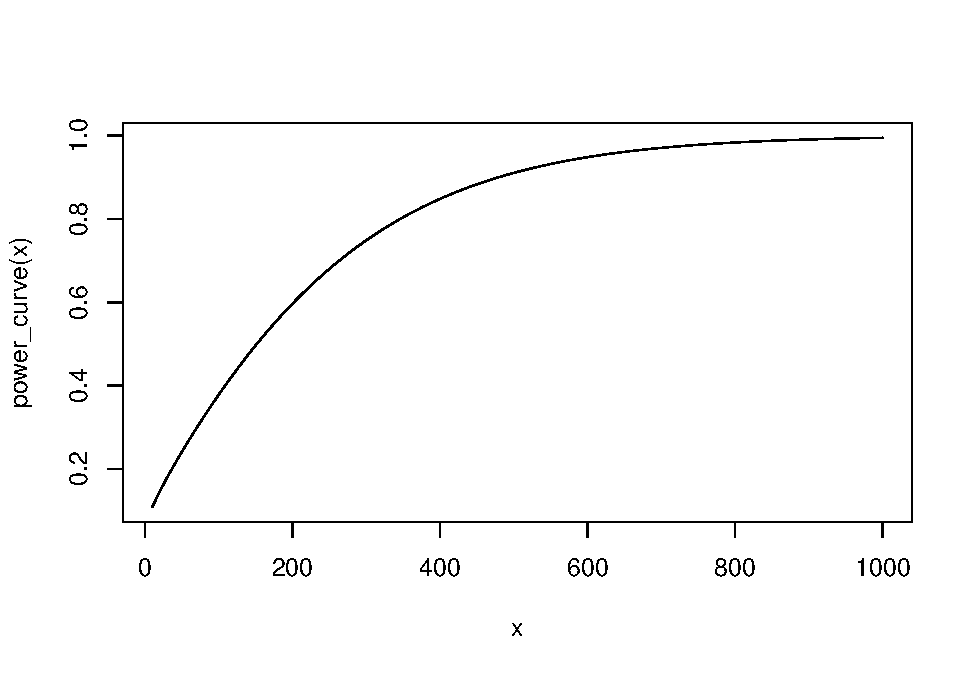
\includegraphics{team_mturk_experiments_files/figure-latex/unnamed-chunk-7-1.pdf}\strut
\end{minipage}\tabularnewline
\begin{minipage}[t]{0.79\columnwidth}\raggedright
\texttt{r\ \#curve(sig\_curve(x),\ 10,\ 1000)\ \#curve(delta\_curve(x),\ 5,\ 20)}\strut
\end{minipage}\tabularnewline
\begin{minipage}[t]{0.79\columnwidth}\raggedright
\#\#\# Experiment 5, threats don't work\strut
\end{minipage}\tabularnewline
\begin{minipage}[t]{0.79\columnwidth}\raggedright
\texttt{r\ e5\_mod\_1\ \textless{}-\ d{[}experiment\_no\ ==\ 5,\ lm(bounding\_box\_score\ \textasciitilde{}\ in\_treatment){]}\ summary(e5\_mod\_1)}\strut
\end{minipage}\tabularnewline
\begin{minipage}[t]{0.79\columnwidth}\raggedright
\texttt{\#\#\ \#\#\ Call:\ \#\#\ lm(formula\ =\ bounding\_box\_score\ \textasciitilde{}\ in\_treatment)\ \#\#\ \#\#\ Residuals:\ \#\#\ \ \ \ \ Min\ \ \ \ \ \ 1Q\ \ Median\ \ \ \ \ \ 3Q\ \ \ \ \ Max\ \#\#\ -12.005\ \ -7.388\ \ -4.123\ \ \ 0.854\ 193.311\ \#\#\ \#\#\ Coefficients:\ \#\#\ \ \ \ \ \ \ \ \ \ \ \ \ \ Estimate\ Std.\ Error\ t\ value\ Pr(\textgreater{}\textbar{}t\textbar{})\ \#\#\ (Intercept)\ \ \ \ 13.552\ \ \ \ \ \ 1.848\ \ \ 7.334\ 6.38e-12\ ***\ \#\#\ in\_treatment\ \ \ -1.938\ \ \ \ \ \ 2.606\ \ -0.743\ \ \ \ 0.458\ \#\#\ -\/-\/-\ \#\#\ Signif.\ codes:\ \ 0\ \textquotesingle{}***\textquotesingle{}\ 0.001\ \textquotesingle{}**\textquotesingle{}\ 0.01\ \textquotesingle{}*\textquotesingle{}\ 0.05\ \textquotesingle{}.\textquotesingle{}\ 0.1\ \textquotesingle{}\ \textquotesingle{}\ 1\ \#\#\ \#\#\ Residual\ standard\ error:\ 18.01\ on\ 189\ degrees\ of\ freedom\ \#\#\ \ \ (2\ observations\ deleted\ due\ to\ missingness)\ \#\#\ Multiple\ R-squared:\ \ 0.002916,\ \ \ Adjusted\ R-squared:\ \ -0.00236\ \#\#\ F-statistic:\ 0.5527\ on\ 1\ and\ 189\ DF,\ \ p-value:\ 0.4582}\strut
\end{minipage}\tabularnewline
\begin{minipage}[t]{0.79\columnwidth}\raggedright
\#\#\# Experiment 6, threats still don't work\strut
\end{minipage}\tabularnewline
\begin{minipage}[t]{0.79\columnwidth}\raggedright
\texttt{r\ e6\_mod\_1\ \textless{}-\ d{[}experiment\_no\ ==\ 6,\ lm(bounding\_box\_score\ \textasciitilde{}\ in\_treatment){]}\ summary(e6\_mod\_1)}\strut
\end{minipage}\tabularnewline
\begin{minipage}[t]{0.79\columnwidth}\raggedright
\texttt{\#\#\ \#\#\ Call:\ \#\#\ lm(formula\ =\ bounding\_box\_score\ \textasciitilde{}\ in\_treatment)\ \#\#\ \#\#\ Residuals:\ \#\#\ \ \ \ Min\ \ \ \ \ 1Q\ Median\ \ \ \ \ 3Q\ \ \ \ Max\ \#\#\ -12.02\ \ -8.64\ \ -6.39\ \ -1.38\ 107.83\ \#\#\ \#\#\ Coefficients:\ \#\#\ \ \ \ \ \ \ \ \ \ \ \ \ \ Estimate\ Std.\ Error\ t\ value\ Pr(\textgreater{}\textbar{}t\textbar{})\ \#\#\ (Intercept)\ \ \ 13.5632\ \ \ \ \ 1.9581\ \ \ 6.927\ 6.99e-11\ ***\ \#\#\ in\_treatment\ \ -0.4096\ \ \ \ \ 2.7842\ \ -0.147\ \ \ \ 0.883\ \#\#\ -\/-\/-\ \#\#\ Signif.\ codes:\ \ 0\ \textquotesingle{}***\textquotesingle{}\ 0.001\ \textquotesingle{}**\textquotesingle{}\ 0.01\ \textquotesingle{}*\textquotesingle{}\ 0.05\ \textquotesingle{}.\textquotesingle{}\ 0.1\ \textquotesingle{}\ \textquotesingle{}\ 1\ \#\#\ \#\#\ Residual\ standard\ error:\ 18.98\ on\ 184\ degrees\ of\ freedom\ \#\#\ Multiple\ R-squared:\ \ 0.0001176,\ \ Adjusted\ R-squared:\ \ -0.005317\ \#\#\ F-statistic:\ 0.02164\ on\ 1\ and\ 184\ DF,\ \ p-value:\ 0.8832}\strut
\end{minipage}\tabularnewline
\begin{minipage}[t]{0.79\columnwidth}\raggedright
\texttt{r\ e6\_mod\_2\ \textless{}-\ d{[}experiment\_no\ \%in\%\ c(5,6),\ lm(bounding\_box\_score\ \textasciitilde{}\ in\_treatment+(Reward\ ==\ "\$0.05")){]}\ summary(e6\_mod\_2)}\strut
\end{minipage}\tabularnewline
\begin{minipage}[t]{0.79\columnwidth}\raggedright
\texttt{\#\#\ \#\#\ Call:\ \#\#\ lm(formula\ =\ bounding\_box\_score\ \textasciitilde{}\ in\_treatment\ +\ (Reward\ ==\ "\$0.05"))\ \#\#\ \#\#\ Residuals:\ \#\#\ \ \ \ \ Min\ \ \ \ \ \ 1Q\ \ Median\ \ \ \ \ \ 3Q\ \ \ \ \ Max\ \#\#\ -12.399\ \ -8.042\ \ -5.148\ \ -0.011\ 193.690\ \#\#\ \#\#\ Coefficients:\ \#\#\ \ \ \ \ \ \ \ \ \ \ \ \ \ \ \ \ \ \ \ \ \ \ Estimate\ Std.\ Error\ t\ value\ Pr(\textgreater{}\textbar{}t\textbar{})\ \#\#\ (Intercept)\ \ \ \ \ \ \ \ \ \ \ \ 13.1730\ \ \ \ \ 1.6439\ \ \ 8.013\ 1.44e-14\ ***\ \#\#\ in\_treatment\ \ \ \ \ \ \ \ \ \ \ -1.1838\ \ \ \ \ 1.9033\ \ -0.622\ \ \ \ 0.534\ \#\#\ Reward\ ==\ "\$0.05"TRUE\ \ \ 0.7731\ \ \ \ \ 1.9034\ \ \ 0.406\ \ \ \ 0.685\ \#\#\ -\/-\/-\ \#\#\ Signif.\ codes:\ \ 0\ \textquotesingle{}***\textquotesingle{}\ 0.001\ \textquotesingle{}**\textquotesingle{}\ 0.01\ \textquotesingle{}*\textquotesingle{}\ 0.05\ \textquotesingle{}.\textquotesingle{}\ 0.1\ \textquotesingle{}\ \textquotesingle{}\ 1\ \#\#\ \#\#\ Residual\ standard\ error:\ 18.48\ on\ 374\ degrees\ of\ freedom\ \#\#\ \ \ (2\ observations\ deleted\ due\ to\ missingness)\ \#\#\ Multiple\ R-squared:\ \ 0.001484,\ \ \ Adjusted\ R-squared:\ \ -0.003855\ \#\#\ F-statistic:\ 0.278\ on\ 2\ and\ 374\ DF,\ \ p-value:\ 0.7575}\strut
\end{minipage}\tabularnewline
\begin{minipage}[t]{0.79\columnwidth}\raggedright
\#\#\# Experiment 7, Even MORE incentive data\strut
\end{minipage}\tabularnewline
\begin{minipage}[t]{0.79\columnwidth}\raggedright
======================================================================================================
Dependent variable:
----------------------------------------------------------------------------------
bounding\_box\_score n=300 n=300 and cellphone n=700 n=700 and cellphone
(1) (2) (3) (4)\strut
\end{minipage}\tabularnewline
\bottomrule
\end{longtable}

in\_treatment -15.895 -14.181 -2.020 -16.466\\
p = 0.116 p = 0.155 p = 0.738 p = 0.105

is\_mobile 50.409***\\
p = 0.003

is\_cellphone 25.693\\
p = 0.426

Constant 33.046*** 27.285*** 21.633*** 32.679***\\
p = 0.00001 p = 0.0002 p = 0.00000 p = 0.00001

\begin{center}\rule{0.5\linewidth}{\linethickness}\end{center}

Data Subset All All x==1\\
Observations 277 277 642 277\\
R2 0.009 0.041 0.0002 0.011\\
Adjusted R2 0.005 0.034 -0.001 0.004\\
Residual Std. Error 83.748 (df = 275) 82.547 (df = 274) 76.188 (df =
640) 83.803 (df = 274) F Statistic 2.494 (df = 1; 275) 5.812*** (df = 2;
274) 0.113 (df = 1; 640) 1.565 (df = 2; 274)
======================================================================================================
Note: \emph{p\textless0.1; \textbf{p\textless0.05; }}p\textless0.01

\begin{Shaded}
\begin{Highlighting}[]
\NormalTok{e7_ate =}\StringTok{ }\NormalTok{d[experiment_no }\OperatorTok\StringTok{ }\KeywordTok{c}\NormalTok{(}\DecValTok{3}\NormalTok{, }\DecValTok{4}\NormalTok{, }\DecValTok{7}\NormalTok{) }\OperatorTok{&}\StringTok{ }\NormalTok{in_treatment }\OperatorTok{==}\StringTok{ }\DecValTok{1}\NormalTok{, }\KeywordTok{mean}\NormalTok{(bounding_box_score, }\DataTypeTok{na.rm=}\NormalTok{T)] }\OperatorTok{-}\StringTok{ }\NormalTok{d[experiment_no }\OperatorTok\StringTok{ }\KeywordTok{c}\NormalTok{(}\DecValTok{3}\NormalTok{, }\DecValTok{4}\NormalTok{, }\DecValTok{7}\NormalTok{) }\OperatorTok{&}\StringTok{ }\NormalTok{in_treatment }\OperatorTok{==}\StringTok{ }\DecValTok{0}\NormalTok{, }\KeywordTok{mean}\NormalTok{(bounding_box_score, }\DataTypeTok{na.rm=}\NormalTok{T)]}

\NormalTok{e7_sd =}\StringTok{ }\NormalTok{d[experiment_no }\OperatorTok\StringTok{ }\KeywordTok{c}\NormalTok{(}\DecValTok{3}\NormalTok{, }\DecValTok{4}\NormalTok{, }\DecValTok{7}\NormalTok{), }\KeywordTok{sd}\NormalTok{(bounding_box_score, }\DataTypeTok{na.rm=}\NormalTok{T)]}


\KeywordTok{power.t.test}\NormalTok{(}\DataTypeTok{delta=}\KeywordTok{abs}\NormalTok{(e7_ate), }
             \DataTypeTok{sd=}\NormalTok{e7_sd, }
             \DataTypeTok{sig.level =} \FloatTok{0.05}\NormalTok{,}
             \DataTypeTok{power =} \FloatTok{0.80}\NormalTok{,}
             \DataTypeTok{alternative =} \StringTok{"one.sided"}\NormalTok{,}
             \DataTypeTok{n =} \OtherTok{NULL}\NormalTok{)}
\end{Highlighting}
\end{Shaded}

\begin{verbatim}
## 
##      Two-sample t test power calculation 
## 
##               n = 17560.84
##           delta = 2.020332
##              sd = 76.13563
##       sig.level = 0.05
##           power = 0.8
##     alternative = one.sided
## 
## NOTE: n is number in *each* group
\end{verbatim}

\end{document}
